\chapter{I/O}
\label{chap:IO}

It is important to understand that the data saved in the file can be in binary
format or human-readable format. With human-readable format, it can be in any
external representation (ASCII, Unicode, \ldots).

 
\section{Encoding schemes}
\label{sec:character_sets}
\label{sec:encoding-scheme}

\begin{itemize}

  \item A {\bf character set} is a collection of graphic characters, which are
  symbols such as letters, numbers, and punctuation marks. 
  
  \item A {\bf set of code points} is a set of hexadecimal values (binary values
  stored in the computer). 
  
  Depending how many characters in a character set, the computer needs to use
  one byte or more to store the code points. With a character set of no more
  than 255 characters, then only 1-byte is needed.
  
  If only 1-byte is used, then it's quite simple. However, if there are more
  than one byte is used, then the order between the bytes to represent one code
  point should be considered. This makes the comparision between characters or
  strings or reading/writing the string data complicated.

  \item  An {\bf encoding schemes} specify how to map each character in a
  character sets to each haxadecimal value in a set of code points.

Examples of encoding schemes: EBCDIC, (7-bit) ASCII, 8-bit ASCII, Windows-1252,
Unicode, ISO 10646.

\end{itemize}

\subsection{Single-byte encoding scheme: ANSI (ANSI\_X3.4-1968 (ISO/IEC
646-1972), ISO/IEC 8859 Latin 1), Windows-1252}
\label{sec:ANSI}

ASCII (ANSI\_X3.4-1968, ISO/IEC 646-1972) is a character-encoding scheme for 128
specified characters \footnote{\url{http://en.wikipedia.org/wiki/ASCII}}. ASCII
character requires only 7-bit for storing code points. 

The ASCII extension (ANSI 8-bit) allows more characters to be added in. 
The first standard for ASCII 8-bit is ISO/IEC 8859 Latin 1 (or simply ISO Latin
1), with characters in the range 128-255 to represent Latin character. Another
popular encoding scheme representing 8-bit character set by Microsoft was
Windows-1252.

IBM PC defined {\it code page 437}, which define the graphical representation
for ASCII characters and some special European characters on the screen. 

\subsection{Multiple-byte encoding scheme: Unicode, ISO 10646}

To deal with more characters (internationalization), newer standards were
developed. MSE (multibyte support extension) was designed to describe
specification on how to add extended character sets to C language. If more than
one byte is required to store code points for characters, then the character set
is called a wide-character set.
Before 1991, the two widely used wide-character sets were Unicode
and ISO 10646 (defined by UCS - Universal Character Set).

The first draft of Unicode was published in 1988 by Joseph D.
Becker.\footnote{\url{http://www.utf8everywhere.org/}} At that time, he believed
16-bit was enough, with the higher byte set to 0 and the lower byte represents
ISO Latin 1 characters.
\footnote{\url{http://www.codeguru.com/cpp/misc/misc/multi-lingualsupport/article.php/c10451/The-Basics-of-UTF8.htm}}
Initially, UNICODE offers support for alphabets from Europe, Africa, Middle
East, Asia (including the unified Han set of East Asian ideograms and the
complete ideograms for Korean Hangul).

\textcolor{red}{Unicode was first designed for 16-bit; while ISO 10646 uses
31-bit}.

From 1991, ISO Working Group and Unicode consortium have coordinated to work on
a single universal standard for multilingual
text.\footnote{\url{http://www.unicode.org/faq/unicode_iso.html}}. However, they
are not exactly the same, as Unicode standard imposes some additional
constraints to make sure cross-platform and applications compatible,
bidirectional algorithms for right-to-left scripts, etc.
\textcolor{red}{Nowadays, Unicode is the widely accepted encoding scheme for
characters}.

Here is the information which Unicode version matches with ISO 10646 version.
\begin{itemize}
  \item Unicode 2.0 (1993): ISO/IEC 10646-1:1993 plus Amendment 5 to 7
  \item Unicode 3.0 (2000): ISO/IEC 10646-1:2000. 
  
The first 65,536 (the Basic Multilingual Plane, or BMP) had entered into common
use before 2000.  Since 2000, China requires all software sold in their country
must support GB 18030, i.e. moving beyond BMP.
    
  \item Unicode 4.0 (2003): ISO/IEC 10646:2003 
  
  \item Unicode 5.0 (2003): ISO/IEC 10646:2003 add Devanagari Letters GGA, JJA,
  DDDA and BBA
  
  \item Unicode 6.0 (2011): ISO/IEC 10646:2011 add Indian Rupee Sign
  \item Unicode 6.1 (2012): ISO/IEC 10646:2012
  \item Unicode 6.2 (2012): ISO/IEC 10646:2012 add Turkish Lira Sign
\end{itemize}

\subsection{Multiple-byte length-variant encoding scheme: UTF-7,
UTF-7.5, UTF-8, UTF-16, UTF-32}

In Unicode:The first 0x10000 code positions is called Basic Multilingual Plane
(BMP). For maximum compatibility, individual Unicode characters are passed
around using 32-bit integer (4-byte per character). However, storing 4-byte per
character is wasteful most of the time.

To improve space saving, different intermediate encoding schemes (Universal
Transformation Format) have been developed (UTF-7, UTF-7.5, UTF-8, UTF-16,
UTF-32). 

UTF-8 is currently the most widely used encode (as the small resulting size of
the string), e.g. filenames in Linux and is supported by all mainstream
webbrowsers. 

\subsection{UTF-8}

The information for UTF-8 is given below.

\begin{verbatim}
   UNICODE            |     UTF-8 (bits representation)
00000000 -- 0000007F: 	0xxxxxxx
00000080 -- 000007FF: 	110xxxxx 10xxxxxx
00000800 -- 0000FFFF: 	1110xxxx 10xxxxxx 10xxxxxx
00010000 -- 001FFFFF: 	11110xxx 10xxxxxx 10xxxxxx 10xxxxxx
00200000 -- 03FFFFFF	111110xx 10xxxxxx 10xxxxxx 10xxxxxx 10xxxxxx
04000000 -- 7FFFFFFF	1111110x 10xxxxxx 10xxxxxx 10xxxxxx 10xxxxxx 10xxxxxx
\end{verbatim}

UTF-8 is length-variant encoding scheme, which means a character can take 1, 2,
3 or 4-bytes of storage, depending on its value (i.e. more bytes are needed as
the values get larger). The last two groups (5-byte and 6-byte) are not used in
the standard to limit the number of byte to 4.

\begin{enumerate}
  
  \item  The first 128 Unicode characters (UTF-8) are the same as those in the
  ASCII encoding, which is good for English characters.

From the bytes greater 127, the meaning are different in UTF-8 as they
represents higher Unicode characters (which is required for internationalization
- locale).

  \item The next 1,920 characters need 2-byte to encode (which covers Latin
  alphabets, Greek, Cyrillic, Coptic, Armenian, Hebrew, Arabic, Syriac, Tana
  alphabets and Combining Diacritical Marks).

To some extent, UTF-8 is backward compatible with ASCII. Most C code
that deals with string on a byte-to-byte basic still works.
  
\end{enumerate}
In November 2003, UTF-8 is limited to encode 1,112,064 valid code points (even
though it can support 1,114,112 characters).
\footnote{\url{http://tools.ietf.org/html/rfc3629}} The last valid code
points is 0x10FFFF (i.e. U+10FFFF).


{\bf HOW TO DECODE ?} The x's are bits to be extracted from the sequence, and
glued together to generate the final numbers. Each byte starts with an escape
sequence (which can be used to easily detect the range of characters).

% So, UTF-8 is {\it variable char length} (1-4 bytes). \textcolor{red}{The whole
% idea of using UTF-8 is that we don't have to change ANY of string-processing
% practices}. It means that we just use the existing functions for ASCII string
% to apply for UTF-8 string.

\begin{mdframed}
UTF-8 is the only Unicode scheme that is compatible with ASCII 7-bit due to its
byte-oriented, i.e. we don't have to change ANY of string-processing practices
(we'll discuss how to read in string data in UTF-8 encoding into a C/C++ program later). 

As UTF-8 is byte stream, there is no byte-order or endianess issue. As a result,
a missing or corrupted byte only affect a single character. Ordering two UTF-8
string can be done using byte-to-byte comparison, faster, rather than using
character-to-character comparison which takes more time to find the character
for a number of bytes.

Using UTF-8 vs. ASCII: With UTF-8, there is no longer a one-to-one mapping
between bytes and characters in a string. So, finding the $n$-th character
requires iterating over the string from the beginning.

\end{mdframed}


\begin{mdframed}

UTF-8 uses the values 100xxxxx in more than 50\% of its representation, but
existing implementation of ISO 2022, 4873, 6429, and 8859 systems mistake these
as C1 control codes. The problem led to the creation of UTF-7,5.

ISO 10646 is an extension to ISO 8859. NOTE: \verb!xterm! utility can handle ISO
10646, but not all Unicode. ISO 10646 defines several character encoding forms:
UCS-2 is for 16-bit (most significant byte first, and represengting characters
in BMP only) and UCS-4 is 32-bit word. UTF-16 is an extension to UCS-2, which
add some more characters to the region (Special Zone) remains unassigned in
UCS-2. Sect.\ref{sec:locale} discuss how to specify a compiled program to
interpret string data in which encoding scheme.

The 8-bit chars of UTF-8 are stripped by many mail gateways because Internet
messages were originally designed as 7-bit ASCII. The problem led to the
creation of UTF-7.
\end{mdframed}

UTF-8 is size-variant, and is byte oriented, and is thus
compatible with \verb!char*!. Thus, sorting a set of UTF-8 strings using
per-byte yield the same result as sorting them per-character by logical Unicode
value; also, there is no byte-order/endianness issue as UTF-8 data is a byte
stream.

UTF-8 is better in recovering from errors compared to UTF-16, i.e. a missing or
corrupted byte in transmission only affect a single character in UTF-8.
Bytes FF and FE never appear in an UTF-8 output, so they can be used to indicate
an UTF-16 or UTF-32 text.

\subsection{UTF-16}
 
UTF-16 is also variable-length, yet the minimum number of bytes is 2. 

UTF-8 is byte-oriented, while UTF-16 is not; i.e. byte-oriented string
operations work on UTF-8 data only. UTF-16 is used in Java's
\verb!String! class, C\#'s \verb!String! class, Win32API
(Sect.\ref{sec:WinAPI}), QT GUI libraries, ICU Unicode library
(Sect.\ref{sec:ICU}). However, using UTF-16 is considered harmful. 


\subsection{UTF-32}

In UTF-32, the number of bytes is always 4. 


\section{I/O: Internal representation to external representation}
\label{sec:internal-representation}

{\it Internal representation} means the representation used by a program while
keeping the text in memory. {\it External representations} are used when text is
stored or transmitted through some communication channel. Examples of external
representations include files waiting in a directory to be read and parsed.

The internal representation refers to how many bytes and the order of the bytes
are used to represent each character in memory (RAM). This is depending on the
programming language and the operating system being used. We will focus on C and
C++.  
Example:
\begin{verbatim}
The value 1 (int) is interpreted as '1' character/string
The value 10 (int) is interpreted as 'A' character/string
\end{verbatim}
The external reperesentation refers to the representation that is stored or
transmitted through some communication channel, i.e. display on terminal or
saving to file. 

The different data types (Chap.\ref{sec:character}) refers to the internal
representation of character-data.
\begin{itemize}
  \item Internal representation (i.e. the data type): \verb!char!,
  \verb!wchar_t!, \verb!std::string!, \verb!char16_t!, \verb!char32_t!:
  specific to machine (litle-endian or big-endian) and O/S (using different
  x-byte of one type on one O/S but y-byte for the same type on a different
  O/S).
  
  \item External representation (i.e. the encoding scheme of data stored in the
  file) which is good for transmission or data exchange between 2 programs:
  ASCII, UNICODE, ISO 10646, etc. (Chap.\ref{sec:encoding-scheme}).
  
\end{itemize}
Traditionally, there is no difference between the two representations,
with \verb!char! as the internal representation and ASCII single-byte
as external representation. Sect.\ref{sec:character_sets} focus on the external
representation of character sets. To work with Unicode, read
Sect.\ref{sec:string_Unicode}. 


I/O functions:
\begin{itemize}
  
  \item  To go from the internal to the external representation (e.g. from
  memory to file), we can use \verb!printf()! or \verb!fprintf()! function, with
  \verb!%d!, \verb!%x! format specifier.

However, the starting address of the memory location (storing the internal
representation) need to be aligned (Sect.\ref{sec:memory_alignment}), otherwise
those functions won't be able to interpret the data. Understanding memory
alignment is very important when programming in C.

  \item To convert from the external to the internal representation,
we use \verb!scanf()! or \verb!fscanf()!, or read the character in some other
ways and then use the functions like \verb!atoi()!, \verb!strtol()!, or
\verb!sscanf()!.
\end{itemize}


Different ways to do I/O
\footnote{\url{http://lemire.me/blog/archives/2012/06/26/which-is-fastest-read-fread-ifstream-or-mmap/}}:
\begin{enumerate}
  \item Low-level read function in Standard C (Sect.\ref{sec:IO_low-level-C})
  
  \item Higher level \verb!fread()! with buffer size in Standard C. Buffers
  reduce number of disk read, but introduce an intermediate step between disk
  and your data.
   
  \item In C++ (<fstream>): \verb!std::ifstream!. Like \verb!fread()!, but with
  a more object-oriented flavor. 
  \item Use {\it memory mapping} (\verb!mmap!): instead of read blocks of data,
  we map the content of the file to a region in memmory. So the file can be
  accessed just like an array via a pointer and the O/S is responsible for
  filling the data from the array back to the disk. It's very fast as the data
  on disk can be mapped directly to the memory without any intermediate buffer.
  But it's  less stable, as it may cause a bus error which crashes your program. 
\end{enumerate}


\section{Special characters}

\begin{enumerate}
  \item \verb!\n! : new line. 
  
\end{enumerate}

\section{Error codes: errno}

\subsection{errno}
\label{sec:error_code}

C language is the widely used one in UNIX environment, despite the popularity of
other languages (C++, Java, Python, Perl). When C and UNIX were developed
(1970s), the concept of {\it exceptions} (Sect.\ref{sec:exception-handling}) (interrupt
the flow of an application when some conditions occur) was new and non-existent.
For reporting errors, C APIs use two common ways
\begin{enumerate}
  \item an error code returned by the API
  \item a specific value (or range of values) is returned by the C API to
  indicate an error, and then the global variable \verb!errno! is set to
  indicate the cause of the problem.
\end{enumerate}

Using \verb!errno! is thread-safe, i.e. each thread has its own \verb!errno!,
defined in \verb!<errno.h>! system header file.
\url{http://www.ibm.com/developerworks/aix/library/au-errnovariable/}
List of all \verb!errno! values:
\url{http://www.ibm.com/developerworks/aix/library/au-errnovariable/} 

\subsection{strerror(), strerror\_r()}
\label{sec:strerror()}
\label{sec:strerror_r()}

To convert the error code to a meaningful string, i.e. human-readable, we use
\verb!strerror(errno)! function, which returns a pointer to a textual
representation of the current \verb!errno! value. This function is not
thread-safe, i.e. for unknown value, it creates an error message in the {\it
static buffer}, and returns the pointer to that buffer. It means that an
additional call to \verb!strerror()! will overwrite the content of that bufer. 

A thread-safe version (since POSIX 1003.1) is \verb!strerror_r()! which accepts
2 additional arguments: a pointer to a buffer, and a buffer-size (counting the
string-terminated NULL character).

\subsection{perror()}
\label{sec:perror()}

NOTE: \verb!perror()! writes the output to the standard-error terminal
(\verb!stderr!)

\begin{lstlisting}
#include <stdio.h>
#include <fcntl.h>
#include <stdlib.h>
#include <errno.h>
#include <string.h>

const char *FILE_NAME = "/tmp/this_file_does_not_exist.yarly";

int main( int argc, char **argv )
{
      int fd = 0;

      printf( "Opening %s...\n", FILE_NAME );	
      fd = open( FILE_NAME, O_RDONLY, 0644 );
      if( fd < 0 ) {
            // Error, as expected.
            perror( "Error opening file" );
            printf( "Error opening file: %s\n", strerror( errno ) );
      }

      return EXIT_SUCCESS;
}

// Thread-safe usage of strerror_r().
void thread_safe( int err )
{
    char buff[256];
    
    if( strerror_r( err, buff, 256 ) == 0 ) {
        printf( "Error: %s\n", buff );
    }
}
\end{lstlisting}


\section{String formatting}

Check Sect.\ref{sec:sprintf}.

\section{I/O to console}

\subsection{printf}
\label{sec:printf}

Becareful when using the specifier, as if you use the one doest not match with
the variable's data type, you will get wrong output, especially when using
inside kernel in CUDA C.

\url{https://en.wikipedia.org/wiki/C_data_types}

\subsection{std::cout, std::cerr}



\section{I/O from consoles}
\label{sec:IO_console}

\verb!cin! ignores the space when reading a string. However, \verb!cin.get()!,
\verb!cin.getline()! and \verb!getline()! read in everything, including
white-sapces. Another important point: \verb!cin.getline()! and \verb!getline()!
consume the delimiter, while \verb!cin.get()! does not. 

\begin{verbatim}
Input of a C-style string variable         Input of a C++ string object
----------------------------------         ----------------------------
cin >> s;                                  cin >> s;
cin.get(s, numCh+1);
cin.get(s, numCh+1,'\n');
cin.get(s, numCh+1,'x');
cin.getline(s, numCh+1);                   getline(cin, s);
cin.getline(s, numCh+1, '\n');
cin.getline(s, numCh+1, 'x');              getline(cin, s, 'x');
\end{verbatim}
\verb!cin! and \verb!cout! accept a C-style string, a C++ string or even an
input or output stream, respectively.

\section{C: <stdio.h> low-level I/O }
\label{sec:IO_low-level-C}

Low-level I/O in C is implemented in glibc library (Sect.\ref{sec:glibc}). These
primitive functions use file descriptors. As it's more flexible and more
convenient to use stream-level I/O, it's suggested to use descriptor-level I/O
under these situations only
\begin{enumerate}
  \item reading binary files in large chunks
  \item reading an entire file into core before parsing it
  \item performing operations other than data transfer
  \item to pass descriptor to a child process (a child process can create its
  own stream using the descriptor it inherits, but it cannot inherit a stream)
\end{enumerate}
\textcolor{red}{To get the file descriptor of a stream, use }\verb!fileno!.
\url{http://www.cs.utah.edu/dept/old/texinfo/glibc-manual-0.02/library_12.html}

\subsection{Open a file: open()}

It returns a new file descriptor for the file with name \verb!filename!, which
is a non-negative integer. If it fails, the value -1 is returned instead.
\begin{verbatim}
int open (const char *filename, int flags[, mode_t mode])
\end{verbatim}
\verb!flags! controls how the file is read
\begin{enumerate}
  \item Use one of these
\begin{verbatim}
O_RDONLY      : read-only
O_WRONLY      : write-only
O_RDWR        : read/write

\end{verbatim}

  \item and combine with one or many of these, e.g. \verb!O_APPEND | O_RDONLY!
\begin{verbatim}
O_APPEND     : write data to the end of file, i.e. extending it
               regardless of the current file position
O_CREAT      : file is created, if not existed
O_EXCL       : if set with O_CREAT, then the file must be non-existing
               otherwise, 'open' fails
O_NOCTTY     : 
O_NONBLOCK
O_TRUNC      : if set with O_WRONLY/O_RDWR, i.e. writing, the file is truncated
               to zero length if existed. This option only works for regular
               file, not for special files (directories or FIFOs)
\end{verbatim}
\end{enumerate}

NOTE: Inside the stream-level functions \verb!fopen! and \verb!freopen!, they
use \verb!open! to do the jobs. 

OBSOLETE 
\begin{verbatim}
int creat (const char *filename, mode_t mode)

 === equivalent to ===
int open (filename, O_WRONLY | O_CREAT | O_TRUNC, mode)
\end{verbatim}

\subsection{Close a file: close()}

\begin{verbatim}
int close (int filedes)
\end{verbatim}
The normal value 0 if success, and -1 if fails. The possible error given by
\verb!errno! error conditions are
\begin{verbatim}
EBADF     : using 'filedes' not a valid descriptor
EINTR     : the call was interupted by a signal
\end{verbatim}

We can avoid 'interuption' by calling
\begin{verbatim}
TEMP_FAILURE_RETRY (close (desc));
\end{verbatim}

\subsection{Read file content}

C language has no direct support for {\it random-access}. Thus, to read in the
middle of the file, we need to create a stream, \verb!seek()! to the middle of
the file, and then read the bytes in sequence.

\subsection{Read a single character: getc(), fgetc(), getchar()}

\url{http://beej.us/guide/bgc/output/html/multipage/getc.html}

We can emulate the pause
\begin{verbatim}
char ch;
ch = std::cin.getc();
\end{verbatim}

\subsection{Read a string from console: gets()}

Read a string from a console/file until a new-line is entered.
NOTE: The newline character is NOT stored as part of the string.

\begin{verbatim}
#include <stdio.h>

char *fgets(char *s, int size, FILE *stream);  //with stdin 
char *gets(char *s);
\end{verbatim}

Using \verb!gets()! is NOT recommended as it has a potential security issue. As
the programmer does not control the maximum buffer that can hold the data, it
cannot detect how much data is input by user, and thus justs read the data until
a newline character is received. If the buffer is next to another data and the
input is overflow, the program will overwrite this data with the 'junk' input
which can cause program crashed.

NOTE: Using \verb!fgets()! is better; but remember it automatically stores the
new line character. It only accepts input (1) with a maximum length, (2) the
newline character can be store if input and the length of the input is less than
the maximum length given for the buffer.

\begin{verbatim}
char s[100];
gets(s);  // read a line (from stdin)
fgets(s, sizeof(s), stdin); // read a line from stdin
\end{verbatim}

\url{http://stackoverflow.com/questions/3302255/c-scanf-vs-gets-vs-fgets}

\subsection{Read a string from console: scanf()}

Avoid using \verb!scanf()!. If not used carefully, it can have the same buffer
overflow problems as \verb!gets()!. Even ignoring that, it has other problems
that make it hard to use correctly.

\url{http://c-faq.com/stdio/scanfprobs.html}




\subsection{mmap()}
\label{sec:mmap()}	


Example:
program A which reads in a 1MB file into a buffer creating with \verb!malloc()!,
and program B which mmaps the 1MB file into memory using \verb!mmap()!.
\begin{itemize}
  \item 
\end{itemize}


\verb!mmap! is great if you have multiple processes accessing data in a read
only fashion from the same file, which is common in the kind of server systems I
write. mmap allows all those processes to share the same physical memory pages,
saving a lot of memory.

mmap has the advantage when you have random access on big files. Another
advantage is that you access it with memory operations (memcpy, pointer arithmetic), without bothering with the buffering.
Normal I/O can sometimes be quite difficult when using buffers when you have
structures bigger than your buffer. 


mmap is also useful for inter process communication.


As people have already mentioned, mmap is quite costly to set up, so it is worth
using only for a given size (varying from machine to machine).


\url{http://stackoverflow.com/questions/258091/when-should-i-use-mmap-for-file-access}

\section{C : stream I/O (FILE object)}
\label{sec:C-stream-IO}

\subsection{header files: }

\begin{enumerate}
  \item stdio.h
  
C language uses \verb!stdio.h! header file, whose functionality descends from
the portable I/O package written by Mike Lesk at Bell Labs (early 1970s).
  
  \item \textcolor{red}{stdio\_ext.h}:

\verb!<stdio_ext.h>! was added to define some extra functions to check a
stream (introduced by Solaris, and nowadays also available in GNU C library)
(Sect.\ref{sec:stdio_ext.h}).

  \item \textcolor{red}{cstdio} (C++ version):

The only reason to use FILE* in C++ (in C++, the header file becomes
\verb!cstdio!) is to allow it to interface with C code taking FILE* as
parameter. 

In C++, only functions from <cstdio> and <cwchar> headers can
interact with FILE objects; and they should be used in the form of pointers
FILE*.  
\end{enumerate}

These I/O functions are fairly low-level by modern standards.
A stream object in C is a pointer to FILE type.
The stream concept in C is reflected in C++ as \verb!iostream!
(Sect.\ref{sec:IO_STL}). 


\begin{mdframed}

FILE is a C object (<stdio.h>), while \verb!std::fstream! is a C++ feature
(Sect.\ref{sec:std::fstream}). There is no performance difference. Only that
\verb!fstream! has better encapsulation, exception safe, and can be treated
generically as a stream (e.g. passing to \verb!cin, cout!). When a std::fstream
goes out of scope it is destructed for you, regardless of whether you forgot to
fstream::close() it.

\end{mdframed}


When the \verb!main()! function of the program is invoked, it already has 3
predefined standard streams (in \verb!<stdio.h>!): stdin, stdout, stderr
(Sect.\ref{sec:standard_stream})

\verb!<stdio.h>! (<cstdio>) and \verb!<stdio_ext.h>! provide all functions to
deal with byte-character (\verb!char!) or wide-character (\verb!wchar_t!), which
are different names or the same name.

\subsection{FILE* object}
\label{sec:FILE}

A FILE* object contains (1) a pointer to the stream's buffer, (2) a file-access
position indicator, (3) flags to indicate error and end-of-file conditions. 


\subsection{Standard stream (stdin, stdout, stderr)}
\label{sec:standard_stream}

\begin{verbatim}
FILE* stdin;
FILE* stdout;
FILE* stderr;
\end{verbatim}
which can be redirect to any files or processes using pipes (|) or redirectional
facilities provided by the shell (e.g. Bash).
\url{http://ftp.gnu.org/old-gnu/Manuals/glibc-2.2.3/html_chapter/libc_12.html_docs}

In GNU C library
\begin{lstlisting}
fclose (stdout);

stdout = fopen ("standard-output-file", "w");
\end{lstlisting}



\subsection{Open file and setbuf()/setvbuf()}

IMPORTANT: Using \verb!fopen, freopen! is not type-safe. It is recommended to
use C++ iostream (Sect.\ref{sec:IO_STL}). Multiple streams can point to the same
file, which is fine for read-only purpose, but it can be a problem for writing.
It's important to use file locking facilities to avoid simultaneous access
(Sect.\ref{sec:file-locking}). However, as each operation already has implicit
file locking, when explicit file locking is used, there is no need for implicit
file locking, and thus using no-locking versions is recommended to boost
performance (Sect.\ref{sec:FILE_nolock}).

To handle large file (greater than $2^{31}$ bytes on 32-bit machines),
\verb!fopen64(), freopen64()! should be used, even though the returned pointer
is still FILE*. A better solution, i.e. keeping using \verb!fopen(), freopen()!,
is to set the macro \verb!_FILE_OFFSET_BITS == 64!. Other operations are
unchanged. If the file is too large that cannot be fit in the main memory (RAM),
then you might use \verb!mmap()! to access portion of the file which is still on
the disk, i.e. reducing RAM usage (Sect.\ref{sec:mmap}).

If we use C style stream, these function generate a stream, connecting
to a given file
\begin{enumerate}
  \item \verb!fopen()!: accept filename as a string (possible UTF-8 if in
  Linux; or must be non-Unicode if in Windows)
  
The C99 version just make the optimization better with \verb!restrict! keyword
(Sect.\ref{sec:pointer_restrict}). Check for failure if a NULL pointer is
returned
\begin{lstlisting}
/* (until C99) */
FILE *fopen( const char          *filename, const char          *mode );

/* fromm C99 */
FILE *fopen( const char *restrict filename, const char *restrict mode );
\end{lstlisting}  

  \item \verb!freopen()!: open a different file with an existing stream
\begin{verbatim}
/* until C99 */
FILE *freopen( const char          *filename, const char          *mode, 
               FILE          *stream );

/* from C99 */
FILE *freopen( const char *restrict filename, const char *restrict mode, 
               FILE *restrict stream );
\end{verbatim}
\end{enumerate}
\verb!mode! is a NULL-terminated string which can be
\begin{verbatim}
                                          IF FILE NOT EXIST
"r"      read         (read froms start)  failure to open
"w"      write        (destroy content)   create new
"a"      append       (write to the end)  create new
                      (regardless of current file position)
"r+"     read+write   (read from start)   error
"w+"     read+write   (destroy content)   create new
"a+"                  (write to end)      create new

// MUST BE AFTER above setting
"b"      binary mode(ONLY ON WINDOWS and optionally combine with above flags)
         As it makes no difference in POSIX system (including GNU system)
          
"x"      (optionally add to "w" or "w+", to indicate that only write to
          non-existing file), i.e. don't overwrite existing file.
   
// GNU libc extension // STRING = the name of the coded character set, //       
  wide-oriented for conversion in-place from/to ,ccs=STRING
\end{verbatim}
At the beginning, any stream is created (opened) as unoriented, and the
orientation (input or output) is decided with the first file operation.
The extension \verb!,ccs=STRING! in GNU libc accepts \verb!STRING! as coded
character sets. If the first operation is wide-character operation, then the
proper function to convert coded character set for the current locale is loaded.
This is not changed, even the locale is changed. Read
Sect.\ref{sec:wide-character_VC++} to know about \verb!,ccs=STRING! in Microsoft
VC++. 

\begin{mdframed}
The maximum number of streams can be open simultaneously is defined in
\verb!FOPEN_MAX! macro (at least 8, including three standard streams -
Sect.\ref{sec:standard_stream}). This value is controlled by \verb!OPEN_MAX!
parameter in POSIX.1; or \verb!RLIMIT_NOFILE! in BSD and GNU.
\end{mdframed}

A FILE object has an internal buffer must be set before starting any I/O
operations. \textcolor{red}{It's recommend to use} \verb!setvbuf()!, instead of
\verb!setbuf(), setlinebuf()! as \verb!setvbuf()! (1) cover the features of
\verb!setbuf(), setlinebuf()!, (2) can detect the successful or failure of the
operation using the returned value, (3) the buffer doesn't have to be
pre-allocated, (4) allow users to select one of the three buffering types to
use. Also, in systems like BSD4.2 BSD 4.3, \verb!setbuf()! always uses a
suboptimal buffer size and should be avoided.

IMPORTANT: \verb!setvbuf()! command should be called after a file associated
with a stream, and {\bf before} any input/output.
\textcolor{red}{Once an I/O is called, calling setvbuf(), setlinebuf() or
setbuf() can cause undefined behavior}.

\begin{mdframed}
NOTE: \verb!(void) setbuf(stream, buf)! is
equivalent to
\begin{verbatim}
(void)setvbuf(stream, buf, buf ? _IOFBF : _IONBF, BUFSIZ);
\end{verbatim}
which is equivalent to
\begin{verbatim}
int setvbuf(stream, buf, _IOFBF, BUFSIZ);

/* or, if buf is a NULL pointer */

int setvbuf(stream, buf, _IONBF, BUFSIZ);
\end{verbatim}
\url{https://www.securecoding.cert.org/confluence/pages/viewpage.action?pageId=3473594}

\end{mdframed}

I/O operation to harddisk is slow. To control how often the real I/O operation
is done, we need to specify if we use buffers or not (the larger the buffer, the
less I/O operation is required as data can be saved to the buffer for fewer I/O
operations). There are 3 types of buffers, which can be specified via the
\verb!mode! argument using one of the three macros: \verb!_IOFBF! fully buffered
(I/O operation only buffer is full), \verb!_IOLBF! line buffered (I/O only when
a newline is seen on the buffer), and \verb!_IONBF! 'not buffered' (unbuffered,
and I/O operation to be performed immediately on the stream, and the last two
arguments are ignored). The macros are defined in \verb!<stdio.h>!.

\begin{lstlisting}
int setvbuf (FILE *stream, char *buf, int mode, size_t size);
\end{lstlisting}
which returns 0 on success, and non-zero otherwise. If \verb!buf! is NULL, then
the system dynamically allocate the buffer if size \verb!size! (bytes)
[REMEMBER to free it yourself and ONLY do it after the stream is closed]
(Sect.\ref{sec:FILE_close}).
\url{http://en.wikibooks.org/wiki/C_Programming/C_Reference/stdio.h/setvbuf}


A user-allocated buffer \verb!buf! should be pre-allocated at least the size
BUFSIZ bytes. [BUFSIZ is a macro (defined in stdio.h, the good size to use for
the buffer, at least 256. The value is chosen to make the stream I/O efficient]
A better number to use is by calling \verb!fstat! system call, and check the
value of \verb!st_blksize! field of the file attribute.

\begin{verbatim}
/* before C99 */
void setbuf(FILE *stream, char *buf)

/* since C99 */
void setbuf( FILE *restrict stream, char *restrict buf);
\end{verbatim}


Example:
\begin{lstlisting}
FILE *file;
char *buf = NULL;
/* Setup file */
if (setvbuf(file, buf, buf ? _IOFBF : _IONBF, BUFSIZ) != 0) {
  /* Handle error */
}
/* ... */

  char buf[42];
 
  if(setvbuf(stdout, buf, _IOFBF, sizeof buf))
  {
     /* Handle error */
  }
\end{lstlisting}

Example: for standard output (stdout)
\begin{Verbatim}
#include <stdio.h>

int main(){
   char buf[BUFSIZ];

   setbuf(stdout, buf);
   puts("This is tutorialspoint");

   fflush(stdout);
   return 0; // return always at main()
             // 0 = success
}
\end{Verbatim}

\subsection{Close the file}
\label{sec:FILE_close}

We handle the file via the stream-ID (\verb!<stdio.h>! header file)
\begin{enumerate}
  \item \verb!int fclose(FILE*)! : close the file using the stream-ID, any
  buffered output is written and any buffered input is discarded. Return 0 =
  success; otherwise \verb!EOF! = error. 
  
  \item \verb!int fcloseall(void)!: close all open streams
\end{enumerate}
It's important to check for error, as potential errors can occur, e.g. the disk
is full even though the buffer is empty (if you're using NFS - network file
system). 

All open streams are automatically closed properly (and buffers is flushed) if
\verb!exit! is called from \verb!main()!. This is not the case if \verb!abort()!
is called or a fatal signal occur.

\subsection{Save and Rewind file position}

\subsection{-- ftell() and fseek()}


fseek() and ftell() can also work with text and binary mode. However there is an
important restriction in text mode: you should only use fseek() with 0 or a
value previously returned by ftell() (in binary mode you can use whatever value
you want).

As ftell() only returns a long int offset, it can't keep track of the multibyte
state if this would be needed. So using fseek() might loose this state.


\subsection{-- fgetpos() and fsetpos()}

There is another type \verb!fpos_t! to keep the current reading position in the
stream which is the result type of the function \verb!fgetpos()!, and we can use
the value to rewind to that position later using \verb!fsetpos(fpos_t)!
function.

\begin{verbatim}
fpos_t fgetpos()

fsetpos(fpos_t)
\end{verbatim}

On some non-UNIX systems, an \verb!fpos_t! object may be a complex object and
these routines may be the only way to portably reposition a text stream.

The advantage of fgetpos() is that is keeps the full position in the stream,
including its internal state, so that you can restore is later. This works
whether you are in text mode or not.

This is especially important if you are using wide oriented streams or mix
fgetc() and fgetwc().

\subsection{Read/Write/Rewind the file (narrow-character)}
\label{sec:FILE_with-lock}

IMPORTANT: When \verb!+! is used to enable bidirectional I/O of a stream
(read+write), ISO C standard requests that when switching from read to write or
vice versa, you must call \verb!fflush()! or a file positioning function such as
\verb!fseek()! to make sure internal buffers is emptied properly. However, this
is not a limitation when using GNU C library. 
\footnote{\url{http://ftp.gnu.org/old-gnu/Manuals/glibc-2.2.3/html_chapter/libc_13.html\#SEC263}}

\subsection{-- read: }

The function \verb!fgets()! read until (whichever comes first) (1) 'size-1'
characters have been read (as 1 character is reserved for the NULL terminator);
(2) a newline is read; (3) end-of-file EOF.
If it reads up to the new line, it also stores this newline character. Finally,
a NULL (or 0) terminator character is inserted to the string.

\begin{verbatim}
#include <stdio.h>

char * c = fgets(char *str, int size, FILE *stream);
\end{verbatim}

{\bf IMPORTANT}: If the End-of-File is encountered and no characters have been
read, the contents of \verb!str! remain unchanged and a null pointer is
returned.


The function \verb!fscanf()! with the \%s specifier reads until any blank space
and doesn't store it that blank space.
\begin{verbatim}
FILE* ptr;

fscanf(ptr, "%9s", str)
\end{verbatim}

TIPS: Use fread()/fwrite() for binary. maximize chunk size. Use fstreams for
ASCII i/o. 

Example: read the file and print each line to the screen
\begin{verbatim}
#include <stdio.h>

int main()
{
   FILE * pFile;
   char buffer [100];

   pFile = fopen ("myfile.txt" , "r");
   if (pFile == NULL) perror ("Error opening file");
   else
   {
     while ( ! feof (pFile) )
     {
       if ( fgets (buffer , 100 , pFile) == NULL ) break;
       /* send the content to the standard-output console */
       fputs (buffer , stdout);
     }
     fclose (pFile);
   }
   return 0;
}
\end{verbatim}


\subsection{-- write: fread, fputs, fprintf, putc, getc}


TIPS: Use fread()/fwrite() for binary. maximize chunk size. Use fstreams for
ASCII i/o. 

We use \verb!fputs(), fprintf(), putc(), getc()! to write data to a stream.
Depending on what kind of buffer is being selected (see setvbuf()), the I/O
operations can be done immediately or not. To enforce it right away, we use
\verb!fflush(FILE*)! statement. Each operation always issue an implicitly lock
request which can slow down the operation.
It's suggested to use explicit locking (Sect.\ref{sec:FILE_multi-threads}) and
use non-locking stream operations (Sect.\ref{sec:FILE_nolock}).

\begin{mdframed}
putc() and getc() was used to be macros, i.e. very fast execution. Since the
introduction of threads, i.e. thread-safe requirement, they are regular
functions, which is slower.
\end{mdframed}

\subsection{-- rewind}


\subsection{Read/Write/Rewind the file (wide-character)}
\label{sec:FILE_with-lock-wide-character}

As ISO C90 introduced a new type \verb!wchar_t!

Existing functions described in Sect.\ref{sec:FILE_with-lock} cannot handle data
in \verb!wchar_t! and saving to file directly. There are some resolutions

\begin{enumerate}
  \item ISO C90: convert the string in \verb!wchar_t*! into multibyte
  string \verb!char*!, and then use the new string for doing I/O operations.
  \textcolor{red}{This is NOT recommended as the conversion is not trivial and
  can increase the program complexity}

\begin{verbatim}
#include <stdlib.h>

size_t wcstombs (char* dest, const wchar_t* src, size_t max);

#include <cstdlib>
std::size_t wcstombs (char* dest, const wchar_t* src, size_t max);
\end{verbatim}

The convertion process stop until the maximum number of wide-characters to be
converted is \verb!max!, or a NULL-character is reached in \verb!src!. The
NULL-character (Sect.\ref{sec:null-character}) is also translated and stored in
the new string; yet it is not counted in the return value, which is the length
of the string. IMPORTANT: If \verb!max! is reached, then the destination string
\verb!dest! is not NULL-terminated. \textcolor{red}{It's important to compare
the returned value vs. the number of characters in the string (src) to know if
a NULL-character is added to (dest) or not.}

Example:
\begin{Verbatim}
  const wchar_t str[] = L"wcstombs example";
  char buffer[32];


  printf ("wchar_t string: %ls \n",str);

  ret = wcstombs ( buffer, str, sizeof(buffer) );
  if (ret==32) buffer[31]='\0';
  if (ret) printf ("multibyte string: %s \n",buffer);

\end{Verbatim}

   \item ISO C90: the two functions [printf(), scanf()] have two specifier,
   \verb!%C! for character, and \verb!%S! for string in wide-character set.
    NOTE: The regular sring use \verb!%c! and \verb!%s!.
   
   To read line by line in C, we mainly use printf(), and fscanf(). It's noted that
using \verb!ifstream! in C++ is 2x-3x slower than using \verb!FILE*!. 

   \item C94/C95 (Amendment 1 to ISO C90): new functions which have counterparts
   are defined: one to work with narrow-character string/narrow-character, and
   one to work with wide-character string/wide-character. Thus, a single stream
   can be used for either wide operations, or normal operations. The current
   restriction, once the stream FILE* object is created, we MUST decide the
   stream {\bf orientation} (narrow or wide-character) and it cannot be changed,
   untill \verb!freopen()! or \verb!freopen64()! is called to reset the
   orientation.
   
How the orientation is decided?
\begin{itemize}
  \item if \verb!fread(), fwrite()! functions are used, which both are narrow
  character functions, then the stream FILE* object is marked as not
  wide-oriented
  
  \item if any of the wide-character functions are used, the stream is marked as
  wide-oriented
  
  \item use \verb!fwide()! to set the orientation or to query the current
  orientation of the stream pointed by \verb!stream! pointer [thread-safe=YES]
  
Use \verb!mode < 0! to set the stream orientation as narrow-character or
byte-oriented) or any positive value (to indicate wide-character). To query the
current orientation, i.e. not making any change to the stream orientation, then
use \verb!mode=0!.
\begin{verbatim}
#include <stdio.h>
#include <wchar.h>

int fwide (FILE *stream, int mode)
\end{verbatim}
When \verb!mode=0! is used, the sign of the return value indicate the stream
orientation. 
% do the query if \verb!mode = 0!, which returns negative value = narrow, zero =
% not configured at all, positive = wide-oriented.

Example: we can write the function to check the orientation
\begin{verbatim}
void check_orientation(FILE *stream)
{
   int rc;
   rc = fwide(stream,0);      /* check the orientation */
   if (rc<0) {
      printf("Stream has byte orientation.\n");
   } else if (rc>0)  {
      printf("Stream has wide orientation.\n");
   } else {
      printf("Stream has no orientation.\n");
   }
   return;
}
\end{verbatim} 
\end{itemize}

\textcolor{red}{When writing code that uses a stream passed into your function,
remember to check the stream orientation before using it}. 
Example:
\begin{Verbatim}
void
print_f (FILE *fp)
{
  if (fwide (fp, 0) > 0)
    /* Positive return value means wide orientation.  */
    fputwc (L'f', fp);
  else
    fputc ('f', fp);
}
\end{Verbatim}

   
\end{enumerate} 

\subsection{Read/Write in multi-threads}
\label{sec:FILE_multi-threads}

When working with multi-thread applications, a stream can be shared by more than
one threads (Chap.\ref{chap:PThreads}). POSIX standards requires each stream
operation is atomic, i.e. two stream operations for the same streams issued at
the same times are executed sequentially. In other words, each stream has an
internal lock object that each operation implicitly acquired the lock before any
work can be done.

You may also want to do explicitly lock the stream. This is the case when the
atomic operation is not a single I/O operation, but several function calls. To
ensure the atomicity of these calls, a stream locking should be issued before
the first call in the group, and release if (if locked successfull) at the end
of the group call. GNU C library also define these functions to lock the stream.
When explicit locking is used, it is recommended to use the unlocked variants of
the I/O operations (Sect.\ref{sec:FILE_nolock}) to improve the speed as no
locking is required in these functions.

\begin{Verbatim}
// keep requesting to lock the stream, the thread is blocked until 
// the lock was successful 
void flockfile (FILE *stream)

// try to lock, but return the control if the lock request is not successful
int ftrylockfile (FILE *stream)

// unlock the stream
void funlockfile (FILE *stream)
\end{Verbatim}


Example: 2 function calls (fputs, fprintf) as an atomic group
\begin{Verbatim}
FILE *fp;
{
   ...
   flockfile (fp);
   fputs ("This is test number ", fp);
   fprintf (fp, "%d\n", test);
   funlockfile (fp)
}
\end{Verbatim}

NOTE: \verb!fputs()! also issue an implicit locking request, even though
\verb!flockfile()! already issued the locking. Thus, multi calls to
\verb!flockfile()! in a single thread is allowed. This suggests that the
implemented locking mechanism is not simple mutexes (see Parallel Programming
Book). Again, we MUST have the same number of calls to \verb!funlockfile()! by
the same thread to unlock the stream completely. However, there is a catch. A call to
\verb!ftrylockfile()! is not always successful. So, it's important to check the
result of every call to \verb!ftrylockfile()! and keep tracks the number of
successfull calls so that we can use the proper number of \verb!funlockfile()!.

Example:
\begin{verbatim}

if (ftrylockfile (fp) == 0)
{
  fputs ("in foo\n", fp);
  funlockfile (fp);
}
\end{verbatim}




\subsection{Read/Write: unlock, faster}
\label{sec:FILE_nolock}

Each I/O operation in Sect.\ref{sec:FILE_with-lock} has an implicit call to lock
the stream and unlock the stream. Locking operations (explicit or implicit)
don't come for free; even if a lock is not taken. When we know for sure the code
using stream is never used in a context where more than one thread can use the
stream at one time. This is mostly the case for application; BUT not for library
code. 

There are two options
\begin{enumerate}
  \item use the \verb!_unlocked! variants of these stream operations which are
  always have NO lock request
\begin{verbatim}
putc_unlocked()
getc_unlocked()
\end{verbatim}
In case we realy need locking, then explicit locking should be used.

  \item GNU C library (\verb!stdio_ext.h!) provides non-standard functions which
  were first introduced in Solaris to disable the implicit locking or reenable.
  Of course, it doesn't apply to \verb!_unlocked! variants.
  
\begin{verbatim}
#include <stdio_ext.h>

int __fsetlocking (FILE *stream, int type)
\end{verbatim}
with \verb!type! is the state to be set, which can be 
\begin{itemize}	
  \item \verb!FSETLOCKING_INTERNAL!: re-enable implicit locking
  \item \verb!FSETLOCKING_BYCALLER!: disable implicit locking, until
  \verb!FSETLOCKING_INTERNAL! is used
  \item \verb!FSETLOCKING_QUERY! : query the current locking state; the return
  value is either one of the two above options.
\end{itemize}

\end{enumerate}

Example: Use a single locking, and multiple stream operations without locking
request/release.
\begin{Verbatim}
  flockfile (fp);
  while (*buf != '/')
    putc_unlocked (*buf++, fp);
  funlockfile (fp);
\end{Verbatim}


\subsection{stdio\_ext.h}
\label{sec:stdio_ext.h}

Solaris introduced this header file \verb!stdio_ext.h! and is now included in
GNU C library. It defines some useful operations on stream

\begin{verbatim}
  // check if the stream is opened for reading ? (non-zero = YES)
int __freadable (FILE *stream)

int __fwritable (FILE *stream)

  // check the last operation is for reading ? (non-ze
int __freading (FILE *stream)

int __fwriting (FILE *stream)
\end{verbatim}

% \subsection{printf/fscanf: narrow-character and wide-character}
% \label{sec:printf_scanf}




\subsection{Checking end-of-file}

A very common error when using \verb!feof(file)! to check for end of file is
\begin{verbatim}
//BUG
FILE * file;
file = fopen('readme.txt', 'r');
while (!feof(file)) {
 //do something;
}
\end{verbatim}

IMPORTANT: The purpose of feof() is NOT the check if the next read will reach
the end of file. The purpose of feof() is to distinguish between a read error
and having reached the end of the file. If fread() returns 0, you must use
feof/ferror to decide whether the error comes from reading issue or just it
reaches the end-of-file. So, we MUST have at least one read-in operation before
using \verb!feof()!.
\begin{verbatim}
//THIS IS CORRECT
FILE * file;
file = fopen('readme.txt', 'r');

int ch = fgetc(ch);

while (!feof(file)) {
 //do something;
}
\end{verbatim}
IMPORTANT: feof() is only useful after fread has returned zero or fgetc has
returned EOF. Before that happens, feof() will always return 0.

It is always necessary to check the return value of a read (either an fread(),
or an fscanf(), or an fgetc()) before calling feof().

\subsection{Read a single character}

We can use \verb!getc(), fgetc(), getchar()!
\footnote{\url{http://beej.us/guide/bgc/output/html/multipage/getc.html}}
\begin{verbatim}
#include <stdio.h>

int getc(FILE *stream);
int fgetc(FILE *stream);
int getchar(void);
\end{verbatim}
The read-in character is actually \verb!unsigned char!, yet they are casted to
\verb!int!. If and end-of-file error occurs, all returns \verb!EOF!.

NOTE: fgetc() and getc() are pretty much equivalent, just the implementations
are different, and \verb!fgetc()! is a little more common. It returns the
current character from the stream, and advance the position indicator to the
next character.

NOTE: \verb!getchar()! is equivalent to \verb!getc(stdin)!, which reads a single
character from the console (Sect.\ref{sec:IO_console}).

\section{C++: STD I/O (cout, cin, cerr, clog)}
\label{sec:std_io}

These functions do I/O to the standard terminal, e.g. output to the screen
or get input from the keyboard

\begin{verbatim}
#include <iostream>

std::cout << string << std::endl;

std::cin >> variable >> var2;

std::cerr << error_msg << std::endl;
\end{verbatim}

\subsection{wcout, wcerr, wclog}



\subsection{with formatting: iomanip}
\label{sec:iomanip}

We can combine with formatting
\begin{verbatim}
#include <iomanip> //setw

  //how to format the number
std::cout << std::setprecision(17) << std::pow(.1, 20) << '\n';

 //reserve how many characters
std::cout << std::setw(17) << std::pow(.1, 20) << '\n'; 

std::cout << std::setw(17) << std::setprecision(17) << std::pow(.1, 20) << '\n'; 

\end{verbatim}

\subsection{redirect output}

In your program, you can redirect all the output to standard I/O to a file,
without changing all the existing \verb!printf()! statements by adding this at
the end of the program. \url{http://en.cppreference.com/w/c/io/freopen}
\begin{Verbatim}
#include <stdio.h>
#include <stdlib.h>

int main(void)
{
    printf("stdout is printed to console");
    if (freopen("redir.txt", "w", stdout) == NULL)
    {
       perror("freopen()");
       fprintf(stderr,"freopen() failed in file %s at line # %d\n", __FILE__,__LINE__-3);
       exit(EXIT_FAILURE);
    }
    printf("stdout is redirected to a file");
    fclose(stdout);
    return EXIT_SUCCESS;
}
\end{Verbatim}

\subsection{new line and flush output}


\textcolor{red}{Flush output}:  std::flush is a manipulator that calls
std::ostream::flush that is, 
\begin{verbatim}
#include <ostream> //std::flush

// using either of this are the same

std::cout << std::flush; 

std::cout.flush();

std::flush(cout);
\end{verbatim}
flush makes sure that the buffer is cleared and the characters are written to
their destination.
\url{http://www.cplusplus.com/reference/ostream/flush-free/}

\textcolor{red}{New line}: To insert new line only, add \verb!\n! at the end of
the string;
\begin{verbatim}
std::cout << "This is a line\n";
\end{verbatim}

\textcolor{red}{New line and flush}: 
\verb!std::endl! automatically (1) insert new line and (2) flush;
\begin{verbatim}
std::cout << "This is a line"  << std::endl;
\end{verbatim}

\section{C++: STL I/O}
\label{sec:IO_STL}

One of the greatest strength of C++ is its Input/Ooutput system, {\bf IO
Streams} (defined in \verb!iostream.h!).

A stream is internally nothing, but a series of characters. The character can be
either a normal character (type: \verb!char!), or a wide character
(\verb!wchar_t!). It's programmers' task to tell how to interpret the string of
characters into meaningful data. IO Stream provides a universal character-based
interface to export data to any medium (e.g. file, another string buffer, etc.)
without requires you to know the details of the output medium.

\begin{mdframed}
There are some performance difference between IO Stream and \verb!stdio!. To
avoid this, there are 2 important things:
\begin{enumerate}
  \item  Avoid using \verb!std::endl!, as it
  implicitly call \verb!std::flush! which causes a major performance problem if
  your code do I/O to the terminal a lot. Here is exactly \verb!std::endl! does 
  \begin{verbatim}
  count << "\n" << std::flush
  \end{verbatim}
  
  \item Disable: \verb!sync_with-stdio()! is a static function of \verb!io_base!
  class.
  \begin{verbatim}
int main () {
    //std::sync_with_stdio (false);
    //std::cout.sync_with_stdio(false);
    std::ios_base::sync_with_stdio (false);
    // ...
}
  \end{verbatim}
\end{enumerate}
\end{mdframed}

\begin{figure}[hbt]
  \centerline{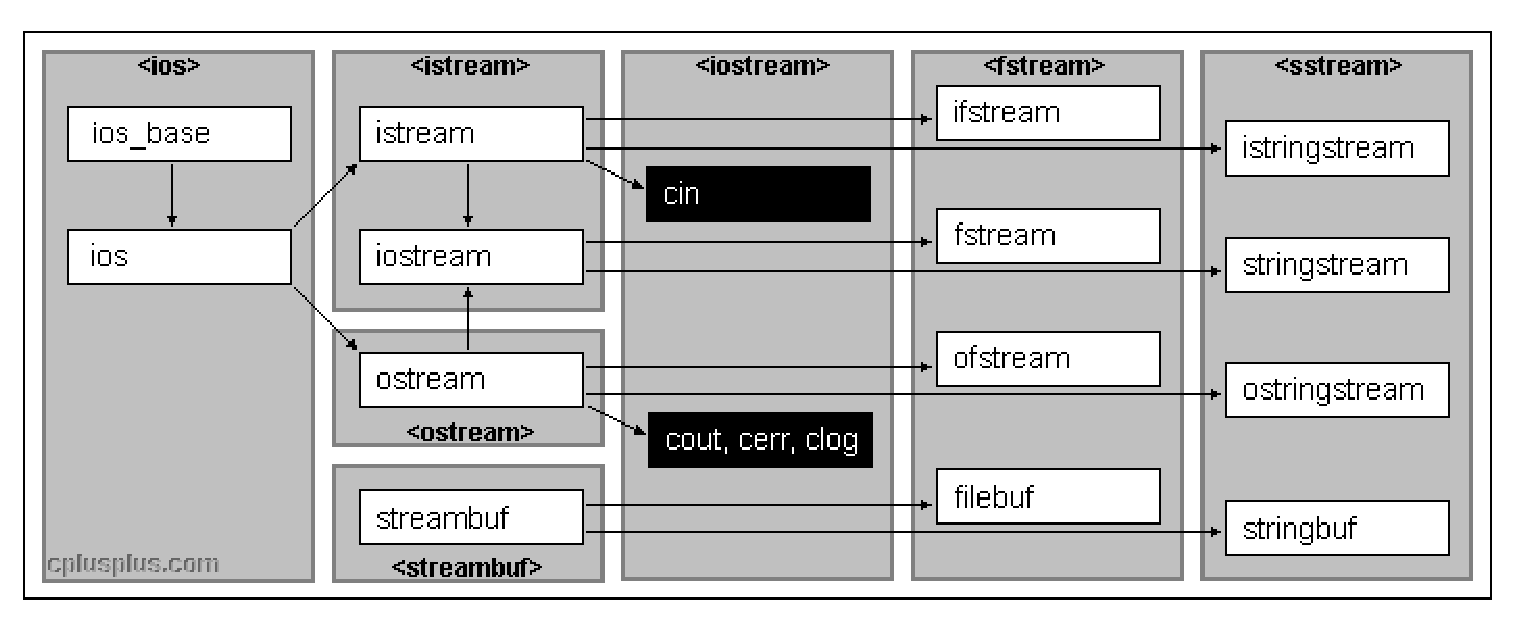
\includegraphics[height=5cm,
    angle=0]{./images/ios_hierarchy.eps}}
  \caption{}
  \label{fig:ios_hierarchy}
\end{figure}

The IO streams class hierarchy is given in Fig.\ref{fig:ios_hierarchy}.  An
important character of IO Stream is serial, we cannot make a random read or
random write to a string. Any built-in data types can be used with IO Streams'
APIs. To export values of user-defined data types, we need to override the {\bf
insertion operator} \verb!<<! to tell how to put objects into the stream, and
the {\bf extraction operator} \verb!>>! to tell how to read objects from the
stream. We can use 
\begin{verbatim}
#include <iostream>
using namespace std;


std::cout << "String to print out"
          << "another line to print out" 
          << std::endl;
\end{verbatim}


To format the parametric output, we use \verb!<iomanip>! (io manipulation). Each
manipulator receives one single argument, and returns one of the six unspecified
type T1 to T6
\footnote{\url{http://publib.boulder.ibm.com/infocenter/comphelp/v9v111/index.jsp?topic=/com.ibm.xlcpp9.aix.doc/standlib/header_iomanip.htm}}
\begin{verbatim}
namespace std {
  T1 resetiosflags(ios_base::fmtflags mask);
  T2 setiosflags(ios_base::fmtflags mask);
  T3 setbase(int base);
     template<class E>
  T4 setfill(E c);
  T5 setprecision(streamsize n);
  T6 setw(streamsize n);
}
\end{verbatim}
\begin{itemize}
  \item How many decimal points to print out after '0'
  \begin{verbatim}
  54.271123 and used setprecision(2) it would print out: 54.27 to the console.
  
  \end{verbatim}
  
  \item
  \begin{verbatim}
cout << setiosflags(ios::fixed) << setiosflags(ios::showpoint);  
  \end{verbatim}
\end{itemize}

\subsection{basic\_streambuf}
\label{sec:basic_streambuf}

\verb!basic_streambfu! is the abstract class, with a number of virtual functions
which are overridden to provide a uniform interface for reading/writing files, strings, etc.

\subsection{pubsetbuf()}

The only required behavior is that stream->pubsetbuf(0, 0) makes the file buffer
unbuffered which you almost certainly don't want. It doesn't make any guarantees
what happens if the arguments are non-null.
In particular, it doesn't guarantee that the buffer being used is the one being
passed! 

\subsection{streambuf}
\label{sec:streambuf}

All stream operations are buffered, with the base class streambuf is used behind
the scenes. It is provided with its own buffer, which size is an implementation
detail.

The stream buffer only affect the maximum number of bytes transferred to or from
the kernel with one syscall. Thus, the ideal buffer size doesn't depend on how
much data you transfer. What is does depend on is

\begin{verbatim}
The overhead cost of syscalls. 
        Higher overhead means you'll want to transfer more data in one go.

The overhead cost of buffer management. Probably larger for larger buffers, if anything.

CPU cache trashing effects. Will strongly favour smaller buffers.
\end{verbatim}
Since (1) works in favour of larger buffers while (2) and (3) work in favour of
smaller buffers, there will be a sweet spot somewhere.


Buffering:

If by default the buffer is very small, increasing the buffer size can definitely improve the performance:

    it reduces the number of HDD hits
    it reduces the number of system calls

Buffer can be set by accessing the underlying streambuf implementation.

\begin{verbatim}
char Buffer[N];

std::ifstream file("file.txt");

file.rdbuf()->pubsetbuf(Buffer, N);
// the pointer reader by rdbuf is guaranteed
// to be non-null after successful constructor
\end{verbatim}


\subsection{ios::rdbuf vs. fstream::rdbuf}

\begin{verbatim}
get (1)	
         streambuf* rdbuf() const;

set (2)	
         streambuf* rdbuf (streambuf* sb);
\end{verbatim}
sets the object pointed by sb as the stream buffer associated with the stream


\subsection{ofstream}

An ofstream by default opens its buffer in output mode only, and either way
you're only passing \verb!std::ios_base::out!, which means the buffer cannot be
read from.

\begin{verbatim}
To fix this you will need to switch to using an fstream and open it with
std::ios_base::in | std::ios_base::out | std::ios_base::binary

You will also need to seek to the start of the file before calling rdbufby
calling seekg(0, std::ios_base::beg).
\end{verbatim}

Use ofstream when textfile is for output only, ifstream for input only, fstream
for both input and output


\subsection{I/O with <istream>, <ostream> or <iostream>: peek(), getline(),
read(), readsome(), ignore()}
\label{sec:iostream}


If we don't care the physical input is a file, a buffer string, or a
console, then we just declare the variable as \verb!std::istream! for input and
\verb!std::ostream! for output. 

\verb!ostream! classes are just wrappers around I/O buffers, and provide
\verb!operator>>! formatting operators. The buffer is provided by an object
derived from \verb!basic_streambuf! (Sect.\ref{sec:basic_streambuf}), which you
can get and set using rdbuf().


There are 2 ways to connect to a file
\begin{verbatim}
// Option 1:
std::ifstream is ("test.txt", std::ifstream::binary);

// Option 2:
std::filebuf fb;
  if (fb.open ("test.txt",std::ios::in))
  {
    std::istream is(&fb);
    while (is)
      std::cout << char(is.get());
    fb.close();
  }
\end{verbatim}
then we can use proper methods to extract data in the form of single character,
a string or a block of data.

It has important functions that can be used in the children classes
\footnote{\url{http://www.cplusplus.com/reference/istream/istream/}}
\begin{itemize}
  \item Read but DON'T extract from the stream
  \begin{verbatim}
  int peek();
  \end{verbatim}
  Read the next character, without extracting. This is useful when you want to
  do parsing
  
  \item Extract character (using C++ string, i.e. you don't have to guess or
  specify the size of the pre-allocate buffer). However, if you read in a file,
  without specifying a \verb!delim! and there is no newline character in the
  file, then \verb!bad_alloc! error may occur.
  \begin{verbatim}
istream& std::getline (istream& is, string& str, char delim);
istream& std::getline (istream& is, string& str);
  \end{verbatim}
which extracts the content from \verb!is! and stores to \verb!str!, until a
delimiter is found (default=newline). NOTE: The delimiter, if found, is
extracted from the stream and is discarded, i.e. not store in \verb!str!.
  
  \item Extract characters (using C-style string):
  \begin{verbatim}
istream& std::istream::getline (char* s, streamsize n );
istream& std::istream::getline (char* s, streamsize n, char delim );
  \end{verbatim}
Extract characters and store them as C-style string \verb!s!, until 
\begin{itemize}
  \item a delimiter is read (default is newline \verb!'\n'!) or 
  \item $n-1$ characters has been read, and written \verb!s! (the $n$-th
  character is the \verb!null! character which is appended automatically)
  \item the end-of-file is reached, , if this occurs first, the \verb!eofbit!
  flag is set.
\end{itemize}
whichever first. A \verb!null! character (\verb!'\0'!) is automatically
appended, even if an empty string is returned.

If you want to be more flexible, you should use \verb!get()! method, which can
does what \verb!getline()! does, and more options: (1) extract a single
character, (2) put to the streambuffer.

  \item Read a block of data from the input (without checking the content nor
  appending NULL character at the end).
  \begin{verbatim}
  istream& istream::read (char* s, streamsize n);
  streamsize istream::readsome (char* s, streamsize n);
  \end{verbatim}
  extract up to $n$ characters, and store them into the array pointed by $s$.
  \verb!readsome()! is designed to work with some types of asynchronous sources
  that may eventually wait for more characters, as the function return as soon
  as the internal buffer is exhausted, i.e. avoiding potential delays.
  
  \item Extract from the input sequence, but discard them, until (whichever
  come first) $n$ characters or a delimiter is read. Default delimiter is EOF
  (end-of-file)
  \begin{verbatim}
  istream& ignore (streamsize n = 1, int delim = EOF);
  \end{verbatim}
  to focus on the delimiter, i.e. ignore as many as possible, we use 
  \begin{lstlisting}
  #include <limist>
  
  file.ignore(std::numeric_limits<std::streamsize>::max(), '}');
  \end{lstlisting}
  
  
  \item Return the number of characters read by the last {\it unformatted input
  operations} called by : \verb!get!, \verb!getline()!, \verb!read!, or
  \verb!readsome()!
  \begin{verbatim}
  streamsize gcount() const;
  \end{verbatim}
\end{itemize}

For output, similarly, we can use \verb!<ostream>!. And if we want to use the
stream for both input + output, we declare it as \verb!<iostream>!.

\subsection{File I/O with <fstream>, <ifstream>, <ofstream>}
\label{sec:std::fstream}

STL also incldue <fstream> which contains input and output stream classes.
\begin{enumerate}
  \item for input only: \verb!ifstream! class
  \item for output only: \verb!ofstream! class
  \item for input + output: \verb!fstream! class. There's an internal buffer
  object calls {\bf filebuf} that performs input/output  operations on the file
  it's associated with.   
\end{enumerate}
% NOTE: std::ifstream is INEFFICIENT compared to fread. The reason is that
% \verb!fread()! put the whole file into memory. So after \verb!fread()!,
% accessing the buffer is faster. 
Beside the standard way to open a file using \verb!.open()! member function, we
can also directly pass the filename when defining the ofstream object.
However, in C++98, the only way to open a file-stream by passing the filename is
to convert to C-style string.
\begin{verbatim}
	std::string filename("text.out");
#if defined(__CXX_EXPERIMENTAL_CXX0X__) || __cplusplus >= 201103L
	std::ofstream ofile(filename);
#else
	std::ofstream ofile(filename.c_str());
#endif	
\end{verbatim}

Another important thing is in C++11, \verb!ofstream! is movable. 

Example: \verb!ifstream:read()! is buffered, and we just tell how much data we
need to read in each time

{\small \begin{verbatim} 
void readFile()
{
    std::ifstream fin;
    fin.open("largefile.dat", ifstream::binary | ifstream::in);
    // in each of these small read methods, there are at least 1 fin.read()
    // call inside.
    readHeaderInfo(fin);
    readPreference(fin);
    readMainContent(fin);
    readVolumeData(fin);
    readTextureData(fin);
    fin.close();
}
\end{verbatim}}

TIPS: Use fread()/fwrite() for binary. maximize chunk size. Use fstreams for
ascii i/o. The best thing around is stream.getline() which saves you any string
ops if you want to extract data by newline (or any other delimiter). 

{\small \begin{verbatim} 
#include <iostream>
#include <fstream>
#include <streambuf>

ofstream ofs("file.txt" );
streambuf* original = cout.rdbuf();
cout.rdbuf( ofs.rdbuf() );  // cout now writes to the file

...

cout.rdbuf( original );  // MUST restore before quitting
\end{verbatim}}

\subsection{Temporay file}
\label{sec:temporary_file}

\verb!std::tmpfile! creates temporary binary file, open for update (``+wb''
mode). The filename is selected by the system, with guarantee that it's
different from any other existing files in the system.
\begin{verbatim}
FILE *pFile;
pFile = tmpfile ( void ); //the pointer to temporary file handle
 
 //work with pFile

fclose(pFile);
\end{verbatim}

To close and also delete the file, we use \verb!fclose(FILE*)!.  If the programs
terminate normally, whether the files are removed depends on the
library implementation.


We can use \verb!ostream!
\begin{verbatim}
char *tmpname = strdup("/tmp/tmpfileXXXXXX");
mkstemp(tmpname);
ofstream f(tmpname);
\end{verbatim}
NOTE: \verb!mkstemp()! can fail and return -1. So the code should catch that
case.

Here is another way
\begin{verbatim}
#include <stdlib.h>
#include <fstream>
#include <iostream>
#include <vector>

std::string open_temp(std::string path, std::ofstream& f) {
    path += "/XXXXXX";
    std::vector<char> dst_path(path.begin(), path.end());
    dst_path.push_back('\0');

    int fd = mkstemp(&dst_path[0]);
    if(fd != -1) {
        path.assign(dst_path.begin(), dst_path.end() - 1);
        f.open(path.c_str(), 
               std::ios_base::trunc | std::ios_base::out);
        close(fd);
    }
    return path;
}

int main() {
    std::ofstream logfile;
    open_temp("/tmp", logfile);
    if(logfile.is_open()) {
        logfile << "hello, dude" << std::endl;
    }
}
\end{verbatim}

References:
\begin{enumerate}
  \item \url{http://www.cplusplus.com/reference/cstdio/tmpfile/}
  
  \item
  \url{http://stackoverflow.com/questions/499636/how-to-create-a-stdofstream-to-a-temp-file}
\end{enumerate}

\subsection{Using user-defined set of routines}

We define a struct that keep the file-handle and file-name.
\begin{verbatim}
typedef struct {
   FILE* file;
   char* name;
} OBJECTFILE
\end{verbatim}

Then, we write a function to open a file \verb!object_fopen()!
\begin{verbatim}
OBJECTFILE file;
file = object_fopen(filename, "r")
\end{verbatim}
with
\begin{verbatim}
OBJECTFILE
object_fopen(const char* filename, char *mode)
{
  OBJECTFILE file;
  file.file = fopen(filename, mode);
  if (file.file == NULL) {
     char *msg;
     int msg_length;
     msg_length = strlen(filename) + 256;
     msg = (char*) Mallloc(msg_length);
     sprintf (msg, "%d: Error opening file=%s with mode %s from object_fopen",
        getRank(0), filename, mode);
     perror(msg);
     Free(msg);
  }
  
  filename = strdup(filename);
  return file;
}

void object_fclose(OBJECTFILE file)
{
  fclose(file.file);
  Free(file.name);
}   

char* object_read(OBJECTFILE file)
{  
}  
\end{verbatim}

\subsection{istringstream}

A stringstream is basically a string, but you can read/write data to it easily
using \verb!<<! and \verb!>>! operator, just like working with file or
\verb!std:cin!.

A stringstream works essentially like an input/output file stream. The
header file required is \verb!<sstream>!. To declare a stringstream, we do
\begin{verbatim}
#include <sstream>

stringstream ss;
\end{verbatim}

We can write to it or read from it using \verb!<<! or \verb!>>! operator
\begin{verbatim}
std::string myString;
char myChar;

ss << mychar ;
ss << myString;

int myInt;

ss >> myInt;
\end{verbatim}
Example:
\begin{lstlisting}
std::string s = "1 2 3"; // this is the original string
std::istringstream is(s); // this istringstream contains a copy of s
int i,j,k; // variables to write to
is >> i >> j >> k; // now i is 1, j is 2, and k is 3
\end{lstlisting}

To convert the entire stringstream to string
\begin{verbatim}
std::string str = ss.str();
\end{verbatim}


Other member functions from stream can be used with stringstream like
\verb!get!, \verb!getline()!, \verb!read!, \verb!write!, \verb!put()!


\section{Boost::Spirit.Karma (Output)}
\label{sec:boost_spirit_Karma}

Typically, \verb!printf, std::stream! formatting, or \verb!boost::format! have
been used for formatting output data. However, for complicated data structure,
it's hard to develop codes for writing data with proper format. A solution is
using \verb!Spirit.Karma! package from Boost::Spirit library. 


This is in opposite of Spirit::Qi which parse the input data from files into
internal data structure (Sect.\ref{sec:boost_spirit_Qi}).

\section{Boost::Spirit::Qi (Input)}
\label{sec:boost_spirit_Qi}

This is the parser library that we use to build recursive descent parsers
(Sect.\ref{sec:boost_spirit}).

Example:
\url{http://www.codeproject.com/Articles/8516/An-Introduction-to-the-Boost-Spirit-Parser-framewo}
We define a grammar class or struct, by inheriting \verb!boost::spirit::grammar!
class. In this class/struct, say \verb!MyGrammar!, we need to define a nested
struct called \verb!definition! (containing the language description that you
want to parse, i.e. a number of rules, ), and a member function call
\verb!start()! (returning the start rule).


\section{Boost::Spirit::Classic (Input)}
\label{sec:boost_spirit_classic}

This is considered depricated and we should use Boost::Spirit::Qi.

\url{http://www.codeproject.com/Articles/8516/An-Introduction-to-the-Boost-Spirit-Parser-framewo}

\url{http://www.codeproject.com/Articles/8522/Implementing-Semantic-Actions-in-the-Boost-Spirit}

{\small \begin{verbatim} 
struct MyGrammar :
    public boost::spirit::grammar<MyGrammar>
{
public:
    MyGrammar( CParser &parser );
    virtual ~MyGrammar();
    template <typename ScannerT>
    struct definition
    {
    public:
        definition( MyGrammar const &self )
        {
            integer =
                lexeme_d[ (+digit_p) ]
                ;
            factor =
                integer |
                vars |
                '(' >> expression >> ')' |
                ( '-' >> factor ) |
                ( '+' >> factor )
                ;
            term =
                factor >> *( ( '*' >> factor) | ( '/' >> factor ) )
                ;
            expression =
                term >> *( ( '+' >> term ) | ( '-' >> term ) )
                ;
            assignment =
                vars
                >> '=' >> expression
                ;
            var_decl =
                lexeme_d
                [
                    ( ( alpha_p >> *( alnum_p | '_' ) )
                    - vars )[vars.add]
                ]
                ;
            declaration =
                "int" >> var_decl >> *( ',' >> var_decl )
                ;
            baseExpression =
                str_p( "exit" )[*self.m_finishedProcessing] |
                str_p( "mod" ) >> integer |
                declaration |
                assignment |
                '?' >> expression
                ;
        }
        boost::spirit::symbols<int> vars;
        boost::spirit::rule<ScannerT> integer, factor, term,
            expression, assignment, var_decl, declaration,
            baseExpression;
        const boost::spirit::rule<ScannerT> &start() const { return baseExpression; }
    };
    friend struct definition;
private:
    Private::FinishedProcessing *m_finishedProcessing;
};
\end{verbatim}}

NOTE: The grammar is described using EBNF rules.
\begin{itemize}
  \item \verb!lexeme_d!: directive to tell the parser NOT to skip white spaces
  \item \verb!+digit_p!: directive to tell matching one or more numeric
  characters
  \item All the rules defined in the \verb!definition! struct, must also be
  defined in the class \verb!MyGrammar! of type
  \verb!boost::spirit::rule<ScannerT>!.
  \begin{verbatim}
        boost::spirit::rule<ScannerT> integer, factor, term,
            expression, assignment, var_decl, declaration,
            baseExpression;  
  \end{verbatim}
  \item The \verb!start()! function returns the entry point rule,
  i.e. baseExpression.
\end{itemize}

Now, after you have read-in the code in the form of a single string, we give it
to the parser.
\begin{verbatim}
//read-in input-file
//storing the content in 'line' string.

boost::spirit::parse_info<> info;
MyGrammar parser;
info = boost::spirit::parse( line.c_str(), parser, boost::spirit::space_p );
\end{verbatim}
NOTE: We can pass a string, or a pair of iterators for begin and end.



\section{Clang: parsing C/C++/Objective-C/Objective-C++ code}

{\bf Clang} is a powerful, free parser that can be used as a front-end for a
compiler \footnote{\url{http://clang.llvm.org/index.html}}. 

\section{Check file status}

We use the \verb!struct stat! structure which is a system struct that is
defined to store information about a given file. There are different field in
this structure. \url{http://codewiki.wikidot.com/c:struct-stat}

 {\small 
\begin{verbatim}
#include <iostream>
#include <sys/types.h>
#include <sys/stat.h>
#include <fcntl.h>
#include <string>
 using namespace std;

int main() {
     struct stat buf;
     std::string filename(``object.data'')
     stat(filename,&buf);

  cout << buf.st_dev << endl;     
 }
\end{verbatim}
}

Another way is to use \verb!filetest()!
\begin{verbatim}
#include <string>

std::string myfile("input.txt");

if (filetest(myfile.c_str(), S_IFREG) != 0) {
  cout << "File not exist";
}
\end{verbatim}

\section{Serialization (copying object's state)}
\label{sec:Serialization_C_C++}

The process to translate data structure or object state into the format that can
be stored (to harddrive), transfered (via network) and then resurrected later is
called {\bf serialization} (deflating, marshalling). This process is not trivial
if the object has extensive use of references. The reverse process, extracting
data structure from a series of bytes is called {\bf deserialization}
(inflating, unmarshalling).

A serialization need to provide at least 4 methods
\begin{enumerate}
  \item to write the object's data to a file or database
  \item to do RPC (remote-procedure call)
  \item to distribute the object
  \item to detect changes in time-varying data
\end{enumerate}
As we need to transfer the data across network, the implementation need to be
portable, i.e. users don't need to concern about byte-ordering, memory layout,
etc.

Serialization, however, breaks the opacity of abstract data type, i.e. you need
to expose private data member (i.e. data encapsulation).

\textcolor{red}{C/C++ do NOT provide direct support to serialization}. However, you can write
your own code for serialization. MFC (Microsoft Foundation Class) library also
provides serialization support. Another library is Boost.Serialization.

\subsection{Boost.Serialization}

The output file format can be: ASCII, XML, binary. The advantage of XML is
useful in debugging. Also, this format is propertary, so you cannot use it to
exchange data with application that doesn't use Boost.Serialization.

You have a simple class:
\begin{verbatim}
/////////////////////////////////////////////////////////////
// gps coordinate
//
// illustrates serialization for a simple type
//
class gps_position
{
private:
    int degrees;
    int minutes;
    float seconds;
public:
    gps_position(){};
    gps_position(int d, int m, float s) :
        degrees(d), minutes(m), seconds(s)
    {}
};
\end{verbatim}

The main concept of Boost.Serialization is an {\bf archive}, which is a sequence
of bytes representing serialized C++ objects. It means that an object can be
loaded into the archive to be serialize from them or to be loaded from it. 
To save the C++ object state to an archive which connect to a particular output
\begin{verbatim}
// Output archive as text stream.
// Even though it's not a stream, it can be used like a stream via << operator
#include <boost/archive/text_oarchive.hpp> 

// save the archive to standard output
boost::archive::text_oarchive oa(std::cout); 
\end{verbatim}


To restore object data from an archive which reads from file, we can use
\begin{verbatim}
#include <boost/archive/text_iarchive.hpp> 

//read from a text file
std::ofstream file("archiv.txt"); 
boost::archive::text_oarchive oa(file); 
\end{verbatim}


\subsubsection{If you can change the class definition}

You need to modify the class and a method name \verb!serialize()! must be
defined. This method is used for both serializing and restoring. The method
should never be called explicitly, and thus should be declared as private, and
the class \verb!boost::serialization::access! is declared as friend.

\begin{verbatim}
class gps_position
{
private:
    friend class boost::serialization::access;
    
    // When the class Archive corresponds to an output archive, the
    // & operator is defined similar to <<.  Likewise, when the class Archive
    // is a type of input archive the & operator is defined similar to >>.
    template<class Archive>
    void serialize(Archive & ar, const unsigned int version)
    {
        ar & degrees;
        ar & minutes;
        ar & seconds;
    }
...
}
\end{verbatim}

Then to save to text file and to restore the class data
\begin{verbatim}
#include <boost/archive/text_oarchive.hpp>
#include <boost/archive/text_iarchive.hpp>


int main() {
    // create and open a character archive for output
    std::ofstream ofs("filename");

    // create class instance
    const gps_position g(35, 59, 24.567f);

    // save data to archive
    {
        boost::archive::text_oarchive oa(ofs);
        // write class instance to archive
        oa << g;
    	// archive and stream closed when destructors are called
    }

    // ... some time later restore the class instance to its orginal state
    gps_position newg;
    {
        // create and open an archive for input
        std::ifstream ifs("filename");
        boost::archive::text_iarchive ia(ifs);
        // read class state from archive
        ia >> newg;
        // archive and stream closed when destructors are called
    }
    return 0;
}
\end{verbatim}

\subsubsection{If you can't (don't want to) change the class definition}

It means the class doesn't have to be derived from a specific class or implement
a specified member function.

You first need to make all data member public or make the class expose enough
information to reconstruct the class state.
\begin{verbatim}
class gps_position
{
public:
    int degrees;
    int minutes;
    float seconds;
    gps_position(){};
    gps_position(int d, int m, float s) :
        degrees(d), minutes(m), seconds(s)
    {}
};
\end{verbatim}

And then define a new member for Boost.Serialization
\begin{verbatim}
namespace boost {
namespace serialization {

template<class Archive>
void serialize(Archive & ar, gps_position & g, const unsigned int version)
{
//put any data member you want to output here
    ar & g.degrees;
    ar & g.minutes;
    ar & g.seconds;
}

} // namespace serialization
} // namespace boost
\end{verbatim}

Typically, we define two function \verb!save()! and \verb!load()!
\begin{verbatim}
void save() 
{ 
  boost::archive::text_oarchive oa(ss); 
  int i = 1; 
  oa << i; 
} 

void load() 
{ 
  boost::archive::text_iarchive ia(ss); 
  int i = 0; 
  ia >> i; 
  std::cout << i << std::endl; 
} 
\end{verbatim}

\subsubsection{Split load/save}

There are two cases: intrusive and non-intrusive approach:

\textcolor{red}{\bf Intrusive}: We need to include \verb!split_member.hpp!
header file, and then define two separate method \verb!save()! and \verb!load()!
to split the serialization into 2 separate functions.

\begin{verbatim}
#include <boost/serialization/split_member.hpp>
 
template<class Archive>
void save(Archive & ar, const unsigned int version) const
{
    // invoke serialization of the base class 
    ar << boost::serialization::base_object<const base_class_of_T>(*this);
    ar << member1;
    ar << member2;
    ar << member3;
}

template<class Archive>
void load(Archive & ar, const unsigned int version)
{
    // invoke serialization of the base class 
    ar >> boost::serialization::base_object<base_class_of_T>(*this);
    ar >> member1;
    ar >> member2;
    if(version > 0)
        ar >> member3;
}

template<class Archive>
void serialize(
    Archive & ar,
    const unsigned int file_version 
){
    boost::serialization::split_member(ar, *this, file_version);
}
\end{verbatim}

\textcolor{red}{\bf Non-intrusive}: 

We need to include \verb!split_free.hpp! file,
\begin{verbatim}
#include < boost/serialization/split_free.hpp>

namespace boost { namespace serialization {

template<class Archive>
inline void serialize(
    Archive & ar,
    my_class & t,
    const unsigned int file_version
){
    split_free(ar, t, file_version); 
}
}}

\end{verbatim}

\subsubsection{Data member as reference/pointer}

In the \verb!serialize()! member function we have
\begin{verbatim}
{
    // save/load class member variables
    ar & member1;
    ar & member2;
}
\end{verbatim}

If it's for a children class, we have
\begin{verbatim}
{
    // invoke serialization of the base class 
    ar & boost::serialization::base_object<base_class_of_T>(*this);
    // save/load class member variables
    ar & member1;
    ar & member2;
}
\end{verbatim}

If you have a data member which is a reference or a pointer, then how and where
the object being referred to are stored and how they are created, e.g.
\verb!member! data member in our case. REMEMBER: reference is a special kind of
pointer, so we serialize the reference as though it is a pointer 
\begin{verbatim}
class object;
class my_class {
private:
    friend class boost::serialization::access;
    int member1;
    object & member2;
    template<class Archive>
    void serialize(Archive &ar, const unsigned int file_version);
public:
    my_class(int m, object & o) :
        member1(m), 
        member2(o)
    {}
};
\end{verbatim}

Then we define an override
\begin{verbatim}
namespace boost { namespace serialization {
template<class Archive>
inline void save_construct_data(
    Archive & ar, const my_class * t, const unsigned int file_version
){
    // save data required to construct instance
    ar << t.member1;
    // serialize reference to object as a pointer
    ar << & t.member2;
}

template<class Archive>
inline void load_construct_data(
    Archive & ar, my_class * t, const unsigned int file_version
){
    // retrieve data from archive required to construct new instance
    int m;
    ar >> m;
    // create and load data through pointer to object
    // tracking handles issues of duplicates.
    object * optr;
    ar >> optr;
    // invoke inplace constructor to initialize instance of my_class
    ::new(t)my_class(m, *optr);
}
}} // namespace ...
\end{verbatim}


\subsubsection{Class versioning}

If we change the class definition, we can use version to determine how to load
the data. When we serialize a class, we have the option to pass the version
information to it.

When it is loaded from the archive, the version number is passed as an argument
to the loading function, we can check using \verb!file_version!
\begin{verbatim}
{
    // invoke serialization of the base class 
    ar & boost::serialization::base_object<base_class_of_T>(*this);
    // save/load class member variables
    ar & member1;
    ar & member2;
    // if its a recent version of the class
    if(1 < file_version)
        // save load recently added class members
        ar & member3;
}
\end{verbatim}

\subsubsection{Using XML}

\begin{verbatim}
boost::archive::xml_oarchive xmlArchive(oStringStream);

xmlArchive.register_type(static_cast<BaseMessage *>(NULL));
xmlArchive.register_type(static_cast<IncomingTradeMessage *>(NULL));
xmlArchive.register_type(static_cast<InternalRequestInfo *>(NULL));
xmlArchive.register_type(static_cast<InternalTradeTransInfo *>(NULL));

const BaseMessage* myMessage =message;

xmlArchive << make_nvp("Message", myMessage);
\end{verbatim}

\subsubsection{Inheritance}

How Boost.Serialization know the class of the object it serializes has a parent,
or even what that parent is.

\begin{lstlisting}
class MyParent {
public:
	
private:
	int ID;
    friend class boost::serialization::access;
    
	template<class Archive> void serialize(Archive& ar,
       const unsigned int version) 
    {
		ar & BOOST_SERIALIZATION_NVP(ID);
	}	
\end{lstlisting}

\begin{lstlisting}
class ChildClass :: MyParent 
{
public:

private:
	friend class boost::serialization::access;
    template<class Archive> void serialize(Archive& ar,
        const unsigned int version) {
          
           /// what should be here???
           /// check below
    }
}
\end{lstlisting}


To serialize the childen class, we need to tell the compiler 
what the object's parent is and provide a reference to it, you can put this line
at the beginning or the end of the \verb!serialize()! member function of the
children class, depening on how you want to structure the output
\begin{verbatim}
ar & boost::serialization::make_nvp("MyParent",
     boost::serialization::base_object<MyParent>(*this))
\end{verbatim}
\url{http://stuartjames.info/Journal/boost-serialization-for-inherited-objects.aspx}

Another option: the children class need have access to
\verb!boost::serialization::base_object()! function inside the
\verb!serialize()! method.
\begin{verbatim}
#include <fstream>
#include <boost/serialization/export.hpp>
#include <boost/archive/text_oarchive.hpp>

class Foo {
    friend class boost::serialization::access;

    template<class Archive>
    void serialize(Archive & ar, const unsigned int version)
    {
        ar & dummy1;
    }

    int dummy1;

public:
    virtual ~Foo() {}
};


class Bar : public Foo {
    friend class boost::serialization::access;

    template<class Archive>
    void serialize(Archive & ar, const unsigned int version)
    {
        // serialize base class information
        ar & boost::serialization::base_object<Foo>(*this);
        ar & dummy2;
    }

    int dummy2;
};

BOOST_CLASS_EXPORT_GUID(Foo, "Foo")
BOOST_CLASS_EXPORT_GUID(Bar, "Bar")

int main(int argc, char *argv[]) {
    std::ofstream ofs("filename");
    boost::archive::text_oarchive oa(ofs);
    Foo *f = new Bar;
    oa << f;

    return 0;
}
\end{verbatim}

\subsection{ACCU}

\url{http://accu.org/index.php/journals/486}


\section{UTF-16 file data}


\subsection{Library: ICU}
\label{sec:ICU}


International Components for Unicode (ICU) provides a cross-platform,
Unicode-based globalization for handling text data in any formats
\footnote{\url{http://site.icu-project.org/home}}.

\begin{itemize}
  \item convert text data to/from Unicode and nearly any other character sets
  \item compare string: based on Unicode Collation Algorithm plus
  locale-specific comparison rules.
  
  \item format string that represents numbers, date, times, currency according
  to a chosen locale.
  \item regular expression: able to handling text left-to-right (English) or
  light-to-left (Arabic, Hebrew) data
  \item text boundaries: 
\end{itemize}

\begin{mdframed}
Why not using ICU?
\begin{itemize}
  \item APIs do not follow modern C++ design, and do not work well with
  newer versions of standard C++ library
  (Sect.\ref{sec:standard-C++-library})
  
  \item UTF-16 oriented. No support for narrow encoding (e.g. ISO 8859)
  
  \item Message translation tool is far from perfect, which can be done with
  GNU \verb!Gettext! model in Boost.Locale (Sect.\ref{sec:Boost.Locale})
  
\end{itemize}

Why using ICU?
\begin{itemize}
  \item one of the best localization/Unicode libraries available
  \item 
\end{itemize}
\end{mdframed}


Compile and install the library before using:
\footnote{\url{http://stuf.ro/reading-a-utf-8-file-in-c-with-icu}}
\begin{verbatim}
// we use -E -H to preserve the environment variables in 'sudo' mode
./configure --enable-static --prefix=/usr && make && sudo -E -H make install

/* statically linking (need to use g++ even for C-code) */
g++ main.c -o main.o -static -lsicuio -lsicui18n -lsicuuc -lsicudata

/* dynamically linking */
gcc main.c -o main.o `icu-config --ld-flags --ld-flags-icuio`
\end{verbatim}


The new data type is \verb!UChar*!, and string operating functions is the same
as C-library except with a prefix \verb!u_!, e.g. \verb!u_printf, u_fclose!. To
allocate and free the string, the function doesn't change, \verb!free()!.
\begin{verbatim}
UChar* str = (UChar*) malloc(sizeof(UChar) * (fsize + 1));
\end{verbatim}

The file object is \verb!UFILE!, with \verb!u_fopen(), u_fclose()! functions.

Example:
\begin{Verbatim}
#include <stdio.h>
#include <stdlib.h>

#include "unicode/ustdio.h"
#include "unicode/uchar.h"

/**
 * Reads a UTF-8 file and returns an UChar array containing the string read.
 *
 * @param filename the path to the file to be read
 * @param size pointer to a variable in which to store the UTF-8 string length
 *
 * @return UTF-8 string (dynamically allocated; must be freed after usage)
 */
UChar* read_utf8_file(const char* filename, long* size) {
    /* open a UTF-8 file for reading */
    UFILE* f = u_fopen(filename, "r", NULL, "UTF-8");

    /* get the file size */
    long fsize;
    fseek(u_fgetfile(f), 0, SEEK_END);
    fsize = ftell(u_fgetfile(f));
    u_frewind(f);

    /* allocate enough memory to store the whole string plus termination */
    UChar* str = (UChar*) malloc(sizeof(UChar) * (fsize + 1));

    /* read the string into the allocated space */
    for ((*size) = 0; !u_feof(f); ++(*size)) {
        str[*size] = u_fgetc(f);
    }

    /* add NULL termination */
    str[*size] = 0;

    /* close the file resource */
    u_fclose(f);

    return str;
}

int main() {
    /* read the string and its size */
    long size;
    UChar* str = read_utf8_file("utf8_test.txt", &size);

    /* print the string size */
    printf("String size: %ld\n\n", size);

    /* print the UTF-8 string */
    UFILE* u_stdout = u_finit(stdout, NULL, NULL);
    u_fprintf(u_stdout, "%S\n", str);
    u_fclose(u_stdout);

    /* free the allocated string */
    free(str);

    return 0;
}
\end{Verbatim}
\section{UTF-8 file data}

If the file is encoded in UTF-8.

\subsection{Microsoft VC++}
\label{sec:wide-character_VC++}

In Microsoft Visual C++ 2005, we can use \verb!fgets()! to decode UTF-8 encoded
file when we create the stream using an extension \verb!ccs=encoding! to open file using
FILE object (Sect.\ref{sec:C-stream-IO}). However, in Visual C++ 2005, this only
work for opening only, not for writing. Other encoded types are also supported
\begin{verbatim}
"ccs=UNICODE" => UTF-16 (Big endian)
"ccs=UTF-8" => UTF-8
"ccs=UTF-16LE" => UTFS-16LE (Little endian) 
"ccs=ANSI" => ANSI (default encoding of the OS)
\end{verbatim}

%wchar_t* unicode_text = L"こんにちは";
Example: reading in
\begin{verbatim}
wchar_t* unicode_text[100];
FILE* f = fopen("C:\\test.txt", "w,ccs=UTF-8");
// fwprintf(f, L"%s\n", unicode_text);
fgets(f, unicode_text);
fclose(f);
\end{verbatim}


For reading in, if you know the locale, you can set with \verb!locale()!
\begin{verbatim}

wchar_t buffer[1000];
FILE* f = fopen("C:\\test.txt", "r");
fgetws(buffer, 1000, f);
fclose(f);

//MessageBoxW(0, buffer, 0, 0);
wprintf (L"% s ", buffer)
\end{verbatim}
Use \verb!fgetws()! to read-in wide-character string.

\subsection{Boost.Locale}
\label{sec:Boost.Locale}

\url{http://www.boost.org/doc/libs/1_55_0/libs/locale/doc/html/index.html}

Boost.Locale connect C++ locale framework, isostreams, and the powerful ICU
library (Sect.\ref{sec:ICU}). Also, Boost.Locale provide non-ICU localization
support.

As ICU is huge (half a million lines of well-tested code), Boost.Locale only
wraps ICU with a modern C++ interface. The entire ICU is hidden behind opaque
pointer and users have no access to it.
